\documentclass[11pt]{report}
\usepackage[latin1]{inputenc}
\usepackage{amsmath}
\usepackage{amsfonts}
\usepackage{amssymb}
\usepackage{graphicx}
\usepackage{listings}
\usepackage{url}
\usepackage{havannah}
\newcommand{\black}{\texttt{Black}}
\newcommand{\white}{\texttt{White}}
\newcommand{\blacks}{\texttt{Black's}}
\newcommand{\whites}{\texttt{White's}}
\newcommand{\loc}[1]{\texttt{#1}}
\begin{document}

\begin{titlepage}
\begin{center}
UNIVERSITY OF CALIFORNIA\\[0.4cm]
SANTA CRUZ\\[0.75cm]
\textbf{Simulation Learning in Computer Hex*}\\[0.4cm]
\small{A report submitted in partial satisfaction}\\
\small{of the requirements for the degree of}\\[0.4cm]
MASTER OF SCIENCE\\[0.4cm]
in\\[0.5cm]
COMPUTER SCIENCE\\[0.4cm]
by\\[0.4cm]
\textbf{James Pettit}\\[0.4cm]
\today
\end{center}
\vfill
\begin{flushright}
The Report of Simulation Learning in Computer Hex\\
is approved:\\[1cm]
\line(1,0){120}\\
Professor David Helmbold\\[1cm]
\line(1,0){120}\\
Professor Robert Levinson\\[3cm]
\end{flushright}
\small{*Many thanks to David Helmbold, David Doshay, and Charlie McDowell for their advice, patience, and the computational resources required to complete this research.}
\end{titlepage}

\tableofcontents

\newpage

\def\dsp{\def\baselinestretch{1.5}\large\normalsize}
\dsp

\renewcommand*\thesection{\arabic{section}}

\section{Introduction}
Abstract strategy games provide an attractive testbed for artificial intelligence and machine learning applications. The game framework provides immediate feedback on algorithm performance. The choice of game and rules can also be experimentally chosen for a variety of difficulty and computational complexity levels. Starting with mathematical game theory research, the most common technique for game AI has been brute force search of the tree of legal moves. This technique, highly tuned and optimized, is what led to Chinook's ascendance to World Champion in 1994 and Deep Blue's eventual victory in 1997 over then World-Champion Gary Kasparov. These victories cemented brute force tree search as standard techniques in abstract strategy games, to the point where computers constructing endgame tables have been strong enough to find sequences lasting for hundreds of moves. Kasparov himself suggested a version of Chess that allowed the player to consult a computer for move advice. Chinook went so far as to solve checkers, proving that perfect play will end in a draw. For at least Checkers, Chess, and similar games (Othello, Connect Four), brute force tree search has provided a silver bullet.

The Hivemind system uses a slightly different approach. It directs a probabilistic (Monte Carlo) tree search with learned heuristics. The problem of requiring a strong outside player or expert knowledge is solved using evolutionary learning from games of self-play. Hivemind provides a framework for Monte Carlo Tree Search, with implementations that can play Hex and Go.

\section{Background: The Game of Hex}
Hex is a two player, full-information, abstract strategy game played on an $N$x$N$ grid of hexagons. The players are denoted by colors here \black{} and \white. The object of the game is to form an unbroken chain from one side of the board to the other. Figure \ref{fig:13x13inprogress} shows an example game in progress on a 13x13 board. Figure \ref{fig:13x13finished} shows the final position, \black{} having just played the winning move, with an unbroken chain connecting both his sides. Hex has properties that make it attractive for AI research. Once placed, a piece never leaves the board. The only criterion for a legal move is that the hexagon be unoccupied (empty). Gale '79 proved the game cannot end in a draw, simplifying minimax methods. Nash, one of the inventors of the game, used a strategy stealing argument to prove the existence of a winning strategy for the first player, but the proof is by reduction and offers no insight into the strategy itself. Solutions for all opening positions for 7x7 and 8x8 boards have been found\cite{henderson2009solving}. A good portion, but not all, 9x9 openings have also been solved. Nash proposed 11x11 as the ideal board size, but 13x13 has been more common in competitions, especially as the ability of computer players improves.

Three Hex programs are currently in the running as viable world champions. Gabor Melis' \emph{Six} is the previous world champion (up to 2007). Six uses traditional alpha-beta search with an evaluation function based on an electrical circuit model (proposed by Anshelevich 2002)\cite{anshelevich2002hierarchical}. \emph{Wolve}, from the University Alberta, also uses the Anshelevich algorithm, but more aggressively prunes provably inferior moves. \emph{MoHex}, also from Alberta, is based on the newer Monte-Carlo Tree Search technique, leveraging the open source \emph{Fuego} library. MoHex is the current world-champion, having finished ahead of Wolve in 2009 and 2010.

Hex is very similar to the game of Havannah, another ``connection'' game. It also has similarities to the board game Go (also known as Igo, Weiqi, and Baduk). Go is a much older game than Hex or Havannah, and much research has been done on Go playing algorithms. Hex has simpler rules than Go, but has a similar branching factor and complexity. Much of this thesis will use Hex as a simpler analog for Go, with the techniques discussed being useful for any large branching game played on a regular board.

\begin{figure}
	\begin{HexBoard}[board size=13]
		\HGame{c4,f6,e11,i8,h8,i1,i6,d5,i3,h9,h5,h4,i4,g9,f9,g8,f7,f8,e8}
	\end{HexBoard}
	\caption{13x13 Hex Game, \white{} to play.}
	\label{fig:13x13inprogress}
\end{figure}

\begin{figure}
	\begin{HexBoard}[board size=13]
		\HGame{c4,f6,e11,i8,h8,i1,i6,d5,i3,
				   h9,h5,h4,i4,g9,f9,g8,f7,f8,
				   e8,e9,c10,k8,c9,g6,g7,c11,
				   d10,h6,h7,i5,j5,j4,k4,k3,
				   m2,l3,m3,l4,c6,e11,l5,m4,
				   d11,b7,e6,d12,c12,c7,e7,f5,
				   e5,d9,d8,f4,e4,f3,a2,e3,d6,
				   c3,d3,d4,b5,e2,d2,d1,e1,b13,
				   c13,c5,b6}
	\end{HexBoard}
	\caption{Finished 13x13 Hex Game, \black{}'s play at \loc{b6} gives him an unbroken path from top to bottom.}
	\label{fig:13x13finished}
\end{figure}

\section{Overview of the Thesis}
In Chapter \ref{mcts} we will review the current state of the art in Monte Carlo Tree Search (MCTS). MCTS is a technique to stochastically sample paths through a game-tree. It has been found to work well in games where: the tree is too large to consider brute-force search, no good solution exists to prune ``bad'' nodes, and no good evaluation function exists. Section \ref{bias} covers the current methods of biasing the tree search, including some methods similar to the technique presented in this paper. Chapter \ref{problem} covers why finding a generic way to bias the tree search would be a step forward in MCTS, with a formal definition of biasing the search, allowing a comparison of different but similar techniques. Chapter \ref{solution} presents a way of biasing the tree that can be automatically evolved through self-play, and does not require outside ``expert'' knowledge. Finally Chapter \ref{results} summarizes the technique and its usefulness, and discusses what can be done in the future to improve and extend it.

\section{State of the Art in Monte Carlo Tree Search}\label{mcts}

\begin{figure}
	\begin{center}
	\begin{HexBoard}[board size=5]
		\HGame{a3,c2}
	\end{HexBoard}
	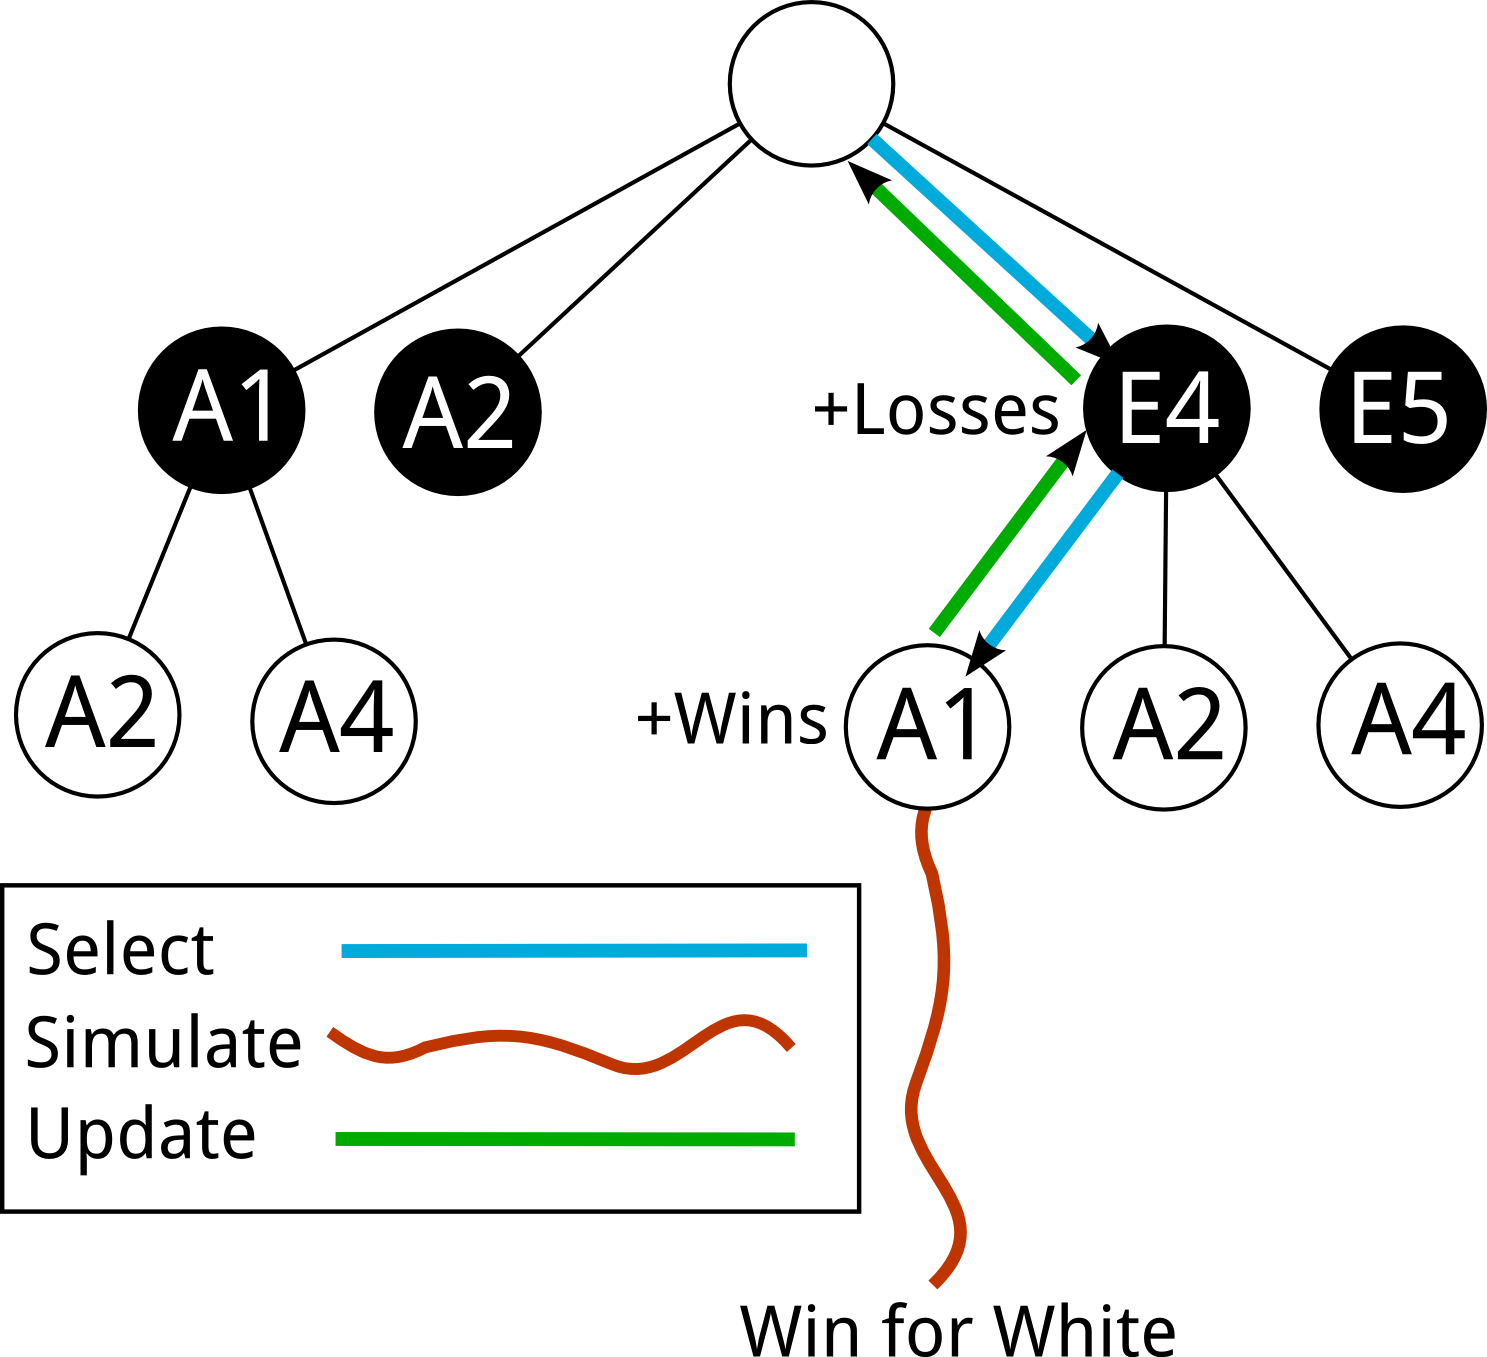
\includegraphics[width=300px]{graphics/tree.png}
	\end{center}
	\caption{Partial MC Search Tree}
	\label{fig:tree}
\end{figure}

As stated, the current top computer Hex player, MoHex, uses the open-source Fuego implementation of Monte-Carlo Tree Search (MCTS)\cite{mohex}. The basic Monte-Carlo technique for Computer Go was proposed by Bru\"{u}gmann\cite{brugmann1993monte}. His program \emph{Mango} effectively used a ``flat'' search tree (1-ply) and simply ran simulations from each candidate move to estimate its value. To contrast, MCTS uses Monte-Carlo simulations to grow a minimax search tree. The UCT algorithm was developed alongside MCTS to direct the growth of the search tree\cite{gelly2006exploration}. At any point, the search can be stopped and the current state of the tree used to select a move to play. Performance of the search is primarily based on three algorithms.
\begin{itemize}
\item{The \emph{selection} policy recursively traverses the tree, selecting good-looking moves for exploration.}
\item{The \emph{simulation} policy randomly or semi-randomly ``plays out'' the game from the current position until a final position.}
\item{The \emph{update} policy modifies the win/loss statistics of nodes based on the simulation results.}
\end{itemize}
Figure \ref{fig:tree} shows a partial Monte-Carlo search tree for the given position. In the example, the selection policy visited the node for \texttt{Black E4}, then \texttt{White A1}. The simulation policy ran, playing out the board with \texttt{E4} occupied by \black\ and \texttt{A1} occupied by \white. This resulted in a loss for \black. The update policy choose to update all nodes along the visited path, incrementing the wins for \white\ moves and incrementing the losses for \black\ moves.

All nodes in the tree correspond to a fixed position, i.e. the occupancy state of the board and which player is next to move. Nodes also have statistics associated with each position - the number of winning simulations performed that used the node, and the total number of simulations that included the node. In general, at each iteration the algorithm will, starting at the root node, recursively traverse the tree until it reaches a leaf node whose estimated value is unknown. A simulation is run from the position of this leaf node and the result used to update all nodes along the path. The algorithm continues for some set number of iterations, each iteration finishing with one simulation.

\begin{lstlisting}[float,frame=single,language=Python,caption=MCTS Algorithm Pseudocode]
def search(root):
  for i in range(simulations):
    step(root)

def play_from(node) returns outcome:
  if node.visits < threshold:
    outcome = simulate(node)
  else:
    child = select(node)
    outcome = play_from(child)
  if outcome is win for node.player:
    node.wins++
  node.visits++
  return outcome
\end{lstlisting}

\subsection{Selection Policy}
The \texttt{select} function defines the selection policy. It must return the child of the given node to step into next. In general, selection must trade off between \emph{exploitation} and \emph{exploration}. It is advantageous to exploit child nodes with high win-rates, to discover possible weaknesses that would result in the opponent winning. Simultaneously, a node with a low win-rate might only have had a few unlucky simulations run through it, resulting in an incorrect value estimate. Nodes with a low number of visits must be explored to see if they result in a high-value position.

One function that balances this trade-off is the Upper-Confidence for Trees algorithm (UCT). UCT incorporates the win-rate of a child with a term that increases in value as the ratio of the child's visits to its parents decreases. Eventually, no matter how bad the estimated value of a position is, it will be re-visited and the estimate updated. UCT has several variations, but the ``pure'' version has been proven to eventually yield the correct minimax value of a position, given an infinite number of simulations\cite{gelly2006exploration}.

The UCT value of a child node is:
\[
	\texttt{child.winrate} + C*\sqrt{\frac{\log{(\texttt{parent.visits})}}{\texttt{child.visits}}}.
\]

The \emph{exploration coefficient}, $C$, can be varied to increase or decrease the level of exploration versus exploitation. Note that a very low value will yield a function that relies almost exclusively on the estimated win-rate of a position, while a high value will visit nodes more equally, placing less emphasis on the estimated value.

\subsection{Simulation Policy}
The \texttt{simulate} function plays out the rest of the game from the current position. The simplest policy plays a legal uniform random move until the game ends (in Hex, when one player has a winning path). The simulation policy has a large effect on the strength of the entire search and, for Go, has a large body of work dedicated to improving it.
Initial research in Computer Go focused on using a strong simulation policy, using expert-derived heuristics to select the next move\cite{chaslot2010adding}. The top Computer Go programs all have complex hand-crafted policies with rules to examine the current position and select a ``good'' move to play, possibly with a stochastic choice between several candidates. Only when none of the rules match do they fall back to a uniform random move. It was quickly found that building a stronger simulation policy does not guarantee better performance when used in the full tree search\cite{gelly2006modification}. A test and check methodology is required, with changes to the simulation policy having unpredictable effects on overall performance.

\subsection{Update Policy}
Once a simulation is finished, the result is used to update the tree statistics. In the basic implementation, only the win and visit statistics along the traversed path are updated. It was quickly discovered that more sophisticated update strategies could be used to keep alternate statistics, and update them at nodes similar to those used in the playout that were not in the path. One simple example of this is the All-Moves-As-First (AMAF) heuristic. Briefly, it leverages the fact that moves played in the simulation could have been played in any order. Thus, a move deep in the simulation could be fictitiously referred to as the ``first'' move. In addition to updating the statistics of the nodes in the path, all siblings corresponding to moves made in the simulation are also updated with a fictitious AMAF win and visit. Variations on AMAF have been tested, including Permutations AMAF, which updates node if any permutation of the simulation contained the node's position, and Some-Moves-As-First, which attempts to restrict the number of siblings updated.

Several methods exist to blend the AMAF results with the ``pure'' results. Formally, a given update policy must define the statistics kept for each node (e.g. \texttt{Pure\_Wins}, \texttt{Pure\_Visits}, \texttt{AMAF\_Wins}, \texttt{AMAF\_Visits}). These counts can be blended into the estimated win-rate used in the UCT selection policy. One simple policy is $\alpha$-AMAF, where a single value, $\alpha \in [0, 1]$, determines the relative weight given to each statistic, e.g.

\[
\texttt{winrate} = \alpha\frac{\texttt{AMAF\_Wins}}{\texttt{AMAF\_Visits}} + (1 - \alpha)\frac{\texttt{Pure\_Wins}}{\texttt{Pure\_Visits}}
\]

Other blending functions include Cutoff and Rapid Action Value Estimation (RAVE)\cite{chaslot2008progressive}. Helmbold and Parker-Wood (2009) have a good summary of the various update policies and blending methods, along with experimental results showing marked improvement over the baseline of pure UCT\cite{helmbold2009all}. One noteworthy conjecture is that there is no ``silver bullet'' update policy. If the simulation policy is random and unbiased, the AMAF updates might be similarly unbiased. However, a simulation policy that preferentially plays certain moves might have an unpredictable effect on which nodes receive AMAF updates. This can then propagate to which nodes are selected during the UCT selection, and have chaotic effects on the search as a whole. 

\subsection{Biasing the Simulation}\label{bias}
Gelly and others have shown that using heuristics in both the expansion and playout policy can prove extremely beneficial\cite{gelly2006modification}\cite{gelly2008achieving}. However, this can require expert knowledge (heuristics) that is hard to obtain or not available for some games (particularly new games). They also found found that improving the performance of playout policy did not guarantee an improvement in the tree search. For example, the playout policy can implicitly prune good moves, never allowing them to be played. In Go, the policy must correctly handle complicated situations like nakade (life and death). If it fails to correctly play out a complex position, the tree might fail to see an opponent response. Much time and energy has been spent on hand-tuning the policies of the top engines to correctly handle complicated tactical situation. If there is some small probability of playing a purely random move, the convergence properties of the UCT algorithm will still hold, but can require a prohibitive amount of playouts to ``find'' the move sequence. In fact, one of the top Go engines, MoGo, uses a near-zero exploration coefficient in the selection policy\cite{gelly2007combining}. This puts most of the control of the search in the hands of the simulation policy.

\section{Problem Statement}\label{problem}
MoGo specifically, and Go programs in general, have the benefit of a rich history of play. Thousands of expert games are available for analysis. Some approaches to improving the simulation policy have focused on using expert games in training weights to direct the playout\cite{chaslot2010adding}. More generally, common patterns are used in a hand-crafted policy to select ``urgent'' moves to play in a local area around the last played move. Hex does have one simple pattern in the form of a bridge\cite{anshelevich2002hierarchical}, but few easy paths to crafting a better simulation policy.

It would be ideal to automatically learn a better playout policy from self-play. The usual process of improvement requires hand-tuned weights that modify the playout policy. Any change must be tested to detect the change in strength it gives. Problematically, small changes in overall algorithm strength require thousands of games of testing to detect. Many times the improvement made by a small change in weight can be so small it will go unnoticed. Automatic weight tuning can improve this process, but still requires thousands of games to test. Recent work in this area has focused on learning weights for a small number of patterns using expert knowledge and reinforcement learning\cite{silver2009monte}. This thesis presents a slightly different approach using evolutionary learning. It solves the problem of requiring a strong outside player or expert knowledge by purely using games of self-play.

\section{Solution}\label{solution}
The simulation policy has the task of quickly selecting a legal move from an arbitrary position. The policy is applied iteratively until the game is finished. Ideally, several thousand games are simulated each second, so the simulation policy must be relatively simple and fast, compared to the full tree search. We consider simulation policies of the following forms:
\begin{itemize}
	\item{Default} - The next move is chosen uniformly from the set of legal moves.
	\item{Uniform local} - The 6-connected (``local'') points surrounding the previous move are examined. The next move is chosen uniformly from any legal moves in this set. If no legal move exists on these 6 points, the default policy is used.
	\item{Uniform local with ``tenuki''} - The tenuki (Japanese: ``play away'') variant includes a small probability ($p=\frac{1}{6}$) of using the default policy, even if a legal local move exists.
	\item{Learned local} - Each local point is matched against a pattern database and assigned a weight. The weight is used as the probability of playing on the given point. Weights are trained over time through self-play using Evolution Strategies.
\end{itemize}

When used at part of a full Monte-Carlo Tree Search, the learned local policy consistently beats both the default policy and the non-learned, uniform local policies. It carries a small cost of computing the pattern hash and looking up weights in the pattern database, but most of the computation is done with offline learning. It is self-bootstrapping, using Evolution Strategies and self-play instead of a strong outside tutor or expert knowledge.

\subsection{Evolution Strategies}\label{estrats}
Evolution strategies (ES) is a collection of algorithms that operate on real-valued vectors. A general form of ES is given here, with some small modifications required for it to represent a biased simulation policy discussed in Section \ref{esmods}. More information on evolution strategies and evolutionary learning in general can be found in Eberhard and Shi's excellent textbook \emph{Computational Intelligence: Concepts to Implementations}\cite{eberhart2007computational}. The Evolution Strategies article on Scholarpedia.org also provides a good introduction to the topic\cite{Beyer:2007}.

\begin{enumerate}
\item A population (usually 20-200 individuals) is generated. In ES, each individual is represented by its vector, often called its ``position'' ($\bf{p}$), a single real-valued ``strategy'' ($\sigma$), and, once evaluation is complete, a single real-valued ``fitness'' attribute ($f$).
\item The algorithm loops, each loop forming one ``generation'':
	\begin{enumerate}
	\item From the $\mu$ parents, generate $\lambda$ children.
		\begin{enumerate}
		\item Each child is created by selecting $P$ parents.
		\item These parents (usually 2 or 3) are \emph{recombined} by averaging their positions component-wise to form the new child position. Similarly, the child's strategy is the average of its $P$ parents.
		\item	The child's strategy ($\sigma$) is \emph{mutated} by a Gaussian distributed random variable.
		\item The child's position is mutated component-wise by a vector of iid Gaussians, one per component of the dimension. These Gaussians are scaled by the strategy. Thus, one individual may mutate more (faster) than another, by using a larger strategy. These strategies mutate along with the positions, allowing the system to evolve the correct mutation weight along with the position.
		\end{enumerate}
	\item The best $b$ performing parents are propagated through without mutation, replacing $b$ children. This is done to preserve well-performing solutions.
	\item Evaluate the fitness of the $\lambda$ children (see \ref{fitness}).
	\item Sort the children by fitness.
	\item Cull the children by selecting only the top $\mu$. These now form the next generation of parents.
	\end{enumerate}
\end{enumerate}

Figure \ref{mutate} shows the differential equations for this evolutionary update. Note that $\sigma$ is multiplied at each time step, and can never reach zero. $\tau$, often called the ``learning rate'', can be scaled up or down to increase or decrease the variance of $\sigma$, a high values will give more mutation, low values less. The initial value of $\tau$ is $\frac{1}{\sqrt{2D}}$, $D$ the dimensionality of the search space. The rate decreases over time, as the number of generations approaches a set maximum, this forces the algorithm to converge, though not necessarily on a suitable solution. This choice of $\tau$ is driven by experimental literature suggesting it works in many cases\cite{Beyer:2007}.

\begin{figure}
\begin{flalign*}
	\tau_{t} = & \frac{1}{\sqrt{2D}} \left(1 - \frac{\textrm{generation}}{\textrm{max generations}}\right) \\
	\sigma_{t} = & \sigma_{t-1} e^{N(0, \tau^2)} \\
	p_{i, t} = & p_{i, t-1} N(0, \sigma_{t}^2)
\end{flalign*}
\caption{Differential equations for $\tau$, $\sigma$, and $\bf{p}$, indexed by time $t$. $D$ is the number of dimensions, i.e. $|\bf{p}|$}
\label{mutate}
\end{figure}

\subsection{Using ES to Bias the Simulation}\label{esmods}
Evolution Strategies evolves a set of real numbered values that are used to bias the playouts. In most applications, the set of values is simply an array, and the array is used directly in fitness evaluation. To apply ES to simulation biasing, an encoding is used that maps from a local pattern to a single 32-bit integer. The 32-bit integer is used to index a single real-valued weight for the pattern. To save space, a growable hashmap is used instead of an array with $2^{32}$ elements. In practice there are less than $2 * 4^6$ possible local patterns so a 16-bit integer could be used. However, this 32-bit hashmap implementation has small overhead and allows space to add properties into the encoding (for example, distance to one side) in the future.

Figures \ref{fig:localpattern} and \ref{fig:encoding} show graphically how a local pattern is mapped to a 32-bit integer. The orange marker denotes the last move played. Around this move any empty vertices are examined for a local response. In the example shown in figure \ref{fig:localpattern}, the sum of the three weights is 11. Thus, vertex A will be selected with probability $P(A) = \frac{6}{11} \approx 0.54$. B will be selected with $P(B) \approx 0.27$ and C with $P(C) \approx 0.18$. Note that $P(A)+P(B)+P(C) = 1$ so one of A, B, or C will be selected. A pattern can have a weight of 0. If so, it will never be selected using the local response policy. If all patterns have weight 0, or if all adjacent vertices are non-empty, play falls back to the default policy (uniform random).

Finally, note that in \ref{fig:encoding} the encoding includes a color bit in the 31st position. This denotes the color to play (either \black\ (1) or \white\ (0)). This bit is important because \black\ and \white\ have conflicting goals of moving, generally, on different diagonals. In fact, by using a reflection and flipping colors, one position can be translated into a similar position for the opposite color. A preliminary implementation was done that used this fact to compress the hashmap with the hope of accelerating learning. In practice this transform is tricky enough to perform that the simpler implementation using color bits was required to ensure correct results.

Using a hashmap slightly complicates the recombination step of ES. The algorithm must now take the superset of patterns (i.e. hashmap keys) from all parents and use those to form the new individual. In practice the hashmap quickly grows to include all possible local patterns after just one generation. Mutation then operates on all values of the hashmap, instead of all values in an array.

\begin{figure}
	\begin{center}
	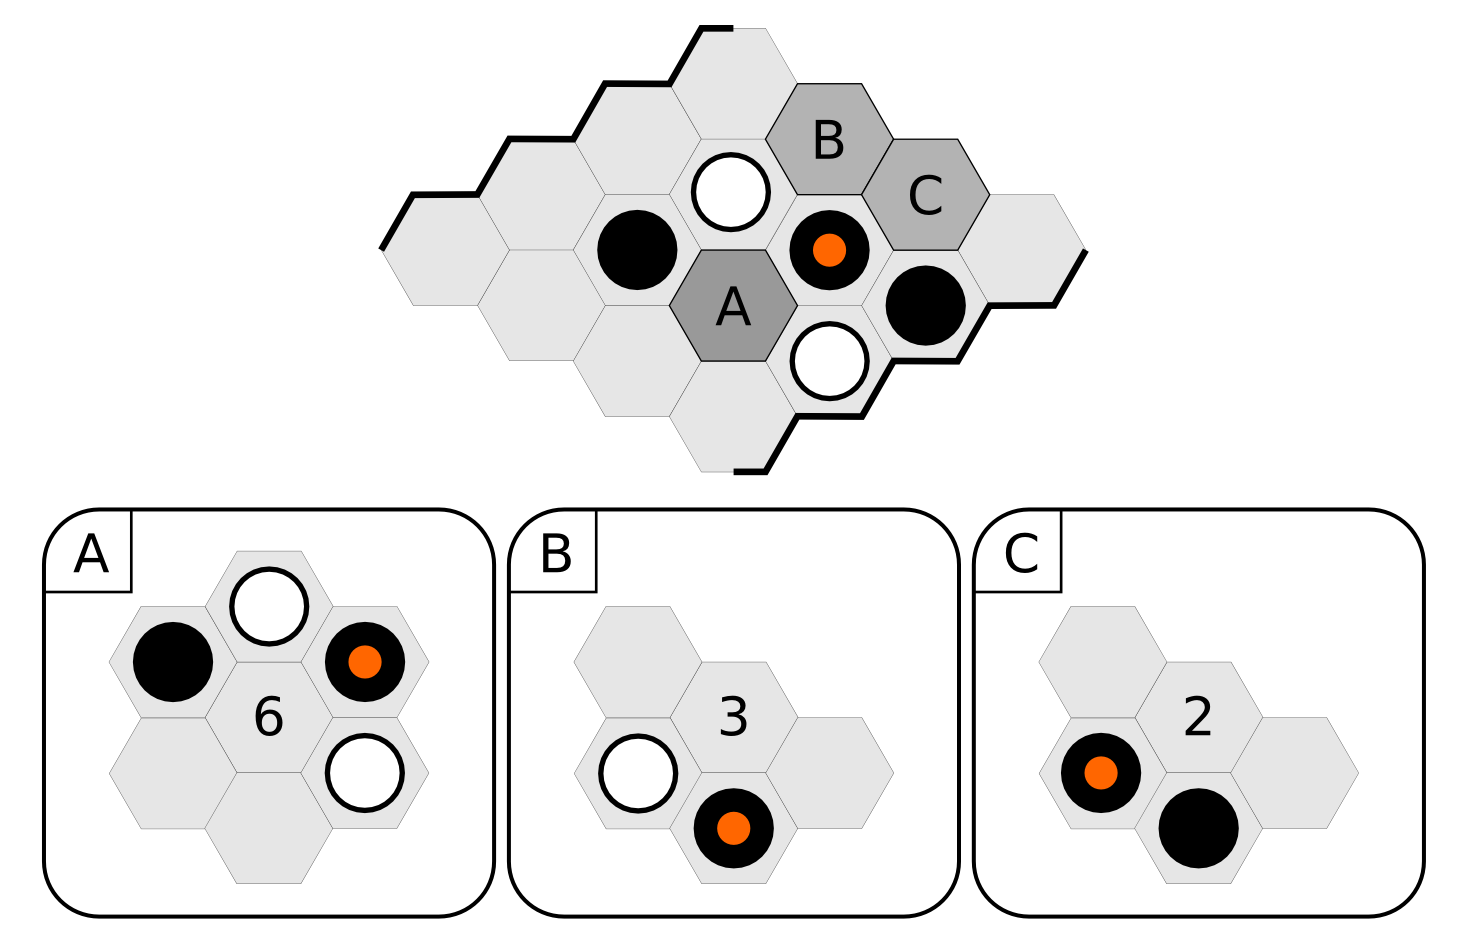
\includegraphics[width=300px]{graphics/local-pattern.png}
	\caption{A 5x5 board with the 3 patterns shown around \blacks\ last move. Example weights are shown in the center vertex.}
	\label{fig:localpattern}
	\end{center}
\end{figure}

\begin{figure}
	\begin{center}
	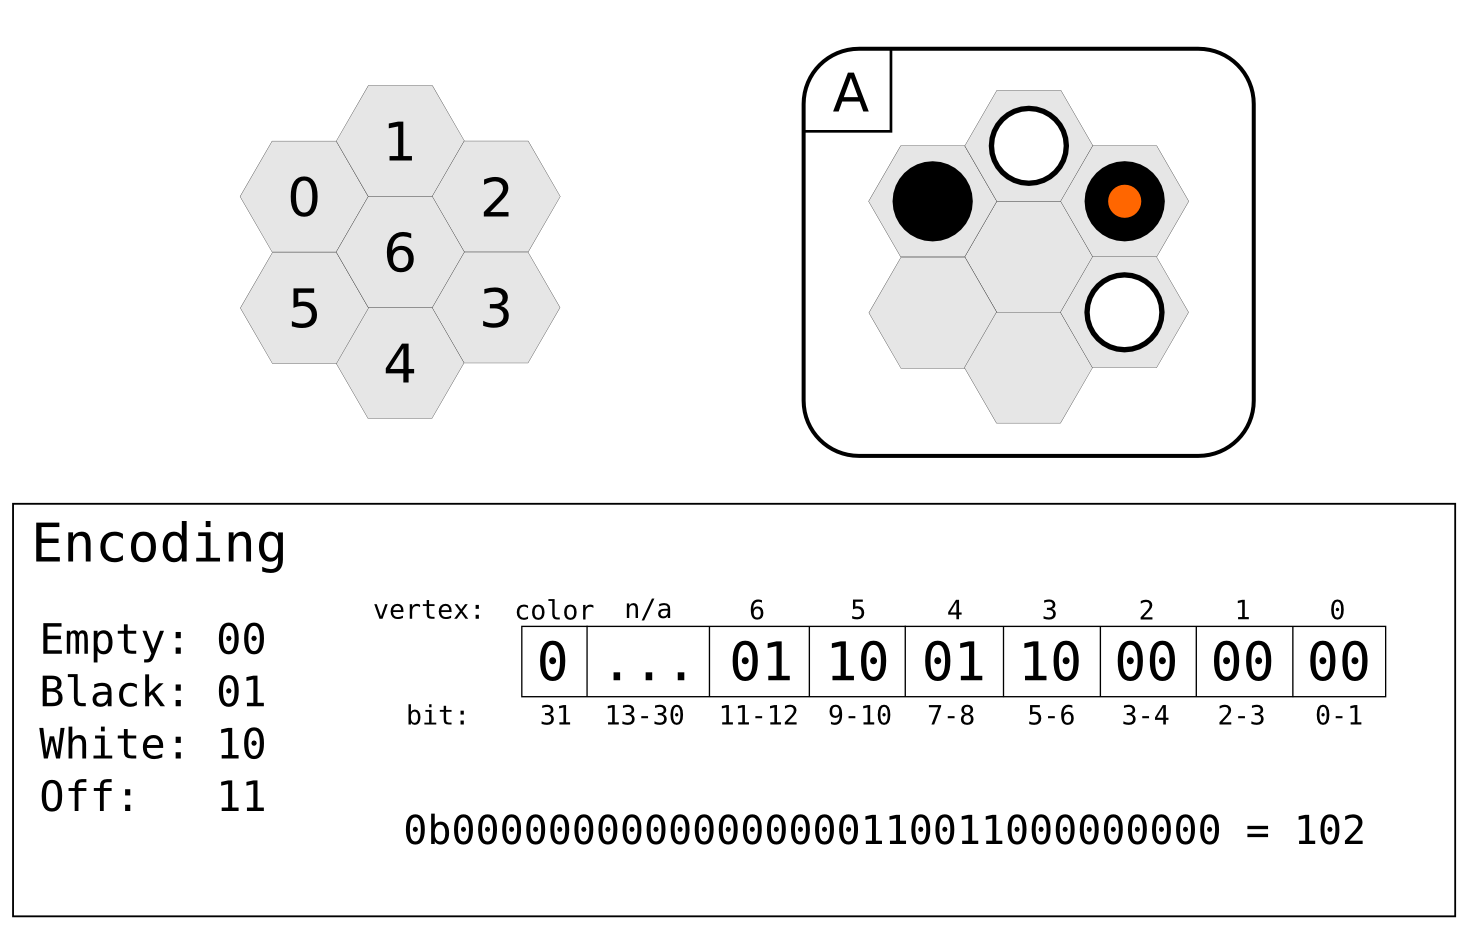
\includegraphics[width=300px]{graphics/weight-pattern-map.png}
	\caption{The encoding from pattern A to a 32-bit integer. Using the weight from figure \ref{fig:localpattern}, the real value 6 would be stored at position 102 in the weight map.}
	\label{fig:encoding}
	\end{center}
\end{figure}

\subsection{Fitness Evaluation}\label{fitness}
The ES population is initialized with $\lambda$ individuals, with uniform random weights in the range $[0, 100]$. In practice, weights are not initialized until a pattern lookup is performed (lazy lookup). Every generation, each individual plays $n$ complete games, each game played against a random individual. Competitors are drawn with replacement from the child population, so a given individual might play the same competitor more than once each generation. At the beginning of each game, one of the two individuals is randomly chosen to play \black, the other to play \white. A swap-safe move was used to play the first move to further equalize first-mover advantage. The winner of a game receives 1 point added to their fitness, the loser has 1 point deducted from their fitness.

\subsection{The Hivemind System}
Hivemind was designed for experiments in learning to play abstract strategy games on a regular board. The system consists of three modules: the evolutionary learning process, a Monte-Carlo based UCT search tree implementation, and a ``game tracker interface''. Blah blah blah Fuego\cite{fuego}. The tracker interface is currently implemented for the games of Hex, Go, and Tic-Tac-Toe. It is designed to be possible to implement many different games in the tracker, abstracting away the learning and search process. Hivemind is open-source software, available at \url{http://github.com/etherealmachine/hivemind}.

\subsubsection{Learning}
The learning module is responsible for driving the evolutionary search process. Currently, Hivemind uses Evolution Strategies (see Section \ref{estrats}), although previous versions experimented with Particle Swarm Optimization. As described earlier, the learning process consists of three steps, iterated once per generation: selection, mutation, and evaluation. In general, the learning module is responsible for finding a strategy (described in Section \ref{esmods}) that generates optimal results during the evaluation step. Evaluation is performed by selecting two individuals from the population and having them play a game against each other, each individual parameterized by their strategy. The individual that wins receives points. During the selection step, individuals are culled based on points received, and the process continues. To play a game, the learning module iteratively calls into the search module with the strategy, until the tracker module reports the game is over. The tracker module is also used to collect the game results.

\subsubsection{Search}
The search module is a simple generic implementation of Monte-Carlo Tree Search, using the UCT algorithm to traverse the tree. Section \ref{mcts} has a description of the MCTS process. The search module uses the Game Tracker to expand the tree and perform the random playouts. The entire source code for search is only about 600 lines of code. Using some extra information from the Game Tracker, search is configurable to use RAVE and AMAF heuristics so a single playout can provide information about the value of multiple nodes.

\subsubsection{Game Tracker}

\section{Results and Conclusions}\label{results}
To test the effects of learning policy weights, the evolution process was ran for 41 generations. This took approximately 2 days using a single core of an Intel Xeon CPU running at 2.80GHz. After training was completed, the best individual from the 41st generation was selected for comparison. This individual was used to bias the simulation policy and compared to the uniform local bias, uniform local bias with a $\frac{5}{6}$th probability of playing locally. The control consisted of uniform random playouts. All players used a slightly modified UCT selection policy that included the variance term suggested by Gelly 2006\cite{gelly2006exploration}. A pure update policy was used, only the nodes directly in the path traversed by UCT were updated with the result of a simulation.

200 games per pair were played, with time controls set at 5 seconds per move. All players have approximately the same performance with regard to simulations per second, so the 5 seconds per move resulted in around 10,000 simulated playouts. A boardsize of 13x13 was used, and to control for the swap rule a swap-safe move was used as the first move for black. Matches were run using the Gomill software\cite{gomill}. Gomill required no modification to work with Hex playing programs.

\begin{figure}
	\begin{center}
		\begin{tabular}{c | c c c}
		 & default & uniform & uniform (tenuki) \\
		\hline
		uniform & 63.50\% & & \\
		uniform (tenuki) & 64.00\% & 50.00\% & \\
		learned & 79.50\% & 81.50\% & 76.00\% \\
		\end{tabular}
	\end{center}
	\caption{All-play-all tournament of the 4 Hivemind variants.}
	\label{fig:results}
\end{figure}
% TODO: run tests using best instead of combined

Learned local play is the clear winner. Interestingly, the addition of a tenuki probability lowers performance in all cases. As expected, uniform local play significantly improves upon pure random playouts. The fact that evolutionary learning can find weights that boost performance versus uniform local in the same manner that uniform local improves upon pure random shows how much further there is to go, and shows the weaknesses of purely random simulations.

As an outside control, MoHex from the University of Alberta was compiled and ran with the default settings\cite{mohex}. Again, 200 games were played. As MoHex is a particularly strong competitor, Hivemind used 100,000 simulations per move. Default time settings for MoHex are 10 seconds, but MoHex uses some time to perform game theoretic search and pruning before the Monte-Carlo phase, and will stop the search early if it believes no better moves will be found. The pre-search can also discover ``must-play'' moves that will be immediately played in lieu of the MCTS. As a result, the time controls are not directly comparable. However, CPU time was tracked and can be used for a cost comparison.

\begin{figure}
	\begin{center}
		\begin{tabular}{c c c c}
		Player 1 & Player 2 & Win-rate & Relative CPU \\
		\hline
		Hivemind Default & MoHex & 6.5\% & 664\% \\
		Hivemind Learned & MoHex & 0\% & 555\% \\
		Hivemind Learned & Hivemind Default & 92.5\% & 131\% \\
		\end{tabular}
	\end{center}
	\caption{Win-rate and relative CPU used of Hivemind versus MoHex. Relative CPU is the ratio of average CPU time per move for Player 1 vs. Player2.}
	\label{fig:relativecpu}
\end{figure}

Learned local patterns provided the only wins against MoHex, with 13 wins out of 200 played. Despite the low performance, MoHex used about 1/6th to CPU time, showing a large distance to cover to get Hivemind up to competition strength. In this series, Hivemind used 100,000 playouts per move, approximately 10 times more than the self-play results. This resulted in an increase in self-play strength, winning 92.5\% of the time when using learned patterns, up from 81.5\% with 10,000 moves. The relative cost for this performance increase was very reasonable, with pattern computation requiring a 31\% overhead.

\subsection{Conclusions}
With infinite time, an unbiased playout policy can find the true minimax value of a position in the game of Hex. In practice, both resources and time are finite. Bias in the playout policy can be extremely useful for improving the overall quality and performance of a Monte-Carlo Tree Search. Evolutionary learning can provide a substantial performance boost over naive patterns. With self-play and evolution, weights can be learned automatically, without requiring expert knowledge or test-and-check tuning. The learning process can be done offline, and the final result can be used with little overhead.

Source code for the Hivemind Computer Hex/Go player is available at \url{http://github.com/etherealmachine/hivemind}. The included README file has instructions on running the evolutionary learning process and using the results.

\bibliography{thesis}
\bibliographystyle{plain}
\end{document}
